% Chapter 1

\chapter{Quark-Gluon Plasma} % Main chapter title

\label{Chapter1} % For referencing the chapter elsewhere, use \ref{Chapter1} 

\section{Strongly interacting matter}
A lot of work has been done so far to study what happened few seconds
after the Big Bang. From the decoupling of neutrinos 
and the nucleosynthesis, the evolution of the Universe is today quite well
understood. Still, we have very little knowledge on what happened before.
Matter was in a very far away state from the one depicted by Quantum Cromodynamics (QCD) at normal temperatures and energy densities. 
Nevertheless, as QCD itself explains, the effective coupling between quarks and gluons depends on the squared transverse momentum $q^2$ exchanged in the interaction. In one loop calculation it can be found that~\cite{Wilson:1970ag}:
\begin{equation}
\alpha_s(q^2)=\frac{\alpha_s (\mu^2)}{1+\alpha_s (\mu^2) \frac{33-2n_f}{12\pi}ln(\frac{-q^2}{\mu^2})}
\end{equation}
where $\mu$ is the momentum scale and $n_f$ is the number of flavors considered. When exploring regions with $|q^2|\rightarrow$ 0, which also corresponds to distances of the order of 1 fermi (hadron size), the strong coupling constant $\alpha_s$ becomes larger. On the other hand, the coupling decreases with increasing $q^2$. This is the so-called {\it asymptotic freedom}, a general feature of non-Abelian gauge theories. Hence, interactions between quarks and gluons become weaker as their mutual distance decreases or as the exchanged momentum increases.
Consequently, matter at very high temperatures or energy densities or at high values of both of them undergoes a phase transition from a state with quarks confined into hadrons into a new state of matter with on-shell quarks and gluons. 
In the primordial universe, quarks and gluons were in this plasma state, their interaction being dominated by the strong fundamental force.
The temperature of the Universe at the time of the Quark-Gluon Plasma (QGP) 
was of hundreds of MeV.
Right after some tens of microseconds, the cooling of this state down to 
a temperature $T \sim$ 150 MeV, lead to the 
creation of structures, irreversibly binding quarks together, inside colorless
hadrons. The QCD matter phase diagram (Fig.~\ref{fig:QCDphase}) predicts the nuclear matter to occur in different phases, depending on the temperature T and the baryo-chemical potential $\mu_{B}$ (defined as the energy needed to increase by one unity the total number of baryons and anti-baryons, $\mu_{B}$ = $\partial$E/$\partial N_B$ and thus being directly related to the baryonic density). 
At low temperatures and for $\mu_{B} \sim 1$ GeV we are in the situation of the ordinary nuclear matter. Raising up the temperatures and/or the chemical potential an intermediate state of hadronic gas is reached, nucleons can interact elastically and form resonances and other hadrons. For even larger values of T and $\mu_{B}$ a transition to the Quark-Gluon Plasma is expected. These were the conditions in which the primordial universe appeared.
The experimental research of this phase of matter started in the second half of the ’80s, with the first fixed target experiments at the SPS at CERN and at the AGS at Brookhaven National Laboratory (BNL). For the first time scientists tried to reproduce in the laboratory such a state of matter, initially through acceleration of light nuclei (Si and S respectively), then moving to heavier nuclei (Pb and Au).\\


\begin{figure}[h!]
\centering
 \includegraphics[width=0.8\textwidth] {FigCap1/QCDphase.jpeg}
\caption{Phase diagram of strongly interacting matter.}
\label{fig:QCDphase}
\end{figure}

Although the transformations in the early universe concerned the interactions among quarks,
this phase transition would never happened if not leaded by macroscopic
collective behaviors, like the system temperature and density. The comprehension of the evolution of this state of matter 
has the promise to become accessible if we understand the thermodynamics laws of the QCD. It is not obvious indeed, nevertheless intriguing,  to understand whether the QCD thermodynamics applies to the fireball created in the laboratory, and whether the emitted hadrons keep a trace of the thermodynamics processes. \\

After SPS, the Relativistic Heavy-Ion Collider (RHIC) at BNL 
has conduced experiments to create hot QCD matter through Au-Au 
collisions with the highest collision energy $\sNN = 200$ GeV, 
one order of magnitude above than the top of SPS energy. 
The Large Hadron Collider (LHC) at CERN is conducing experiments 
along the same line with the highest achievable center-of-mass 
energy of $\sNN = 5.02$ TeV per nucleon-nucleon collision.

\section{Micro bang vs big bang: timescales of expansion, baryonic number}
The system created in the laboratory by colliding
high-relativistic nuclei presents many similarities with 
the matter of the primordial universe, but also some differences. 
A Hubble-like expansion drives the 
evolution of the system after the collisions in the laboratory and the fireball undergoes different phases: 
\begin{itemize}
\item Pre-equilibrium phase: parton scatterings produce a large number of partons; they interact among them leading the fireball thermalizing at a time of $\sim$ 0.6-1 fm/c with the creation of high-$\pt$ probes (heavy quarks, photons) and low-$\pt$ particles;
\item QGP phase: with high-energy collisions, if the temperature inside the fireball exceeds the critical temperature $T_{\rm c}$, the system is in a deconfined phase with partonic degrees of freedom. While the phase of QGP in the early universe lasted
tens of microseconds, due to the interplay of gravity and
radiative pressure of the expanding matter, in the plasma created in the laboratory 
there is no gravity to slow down the expansion, which lasts for a period of
the order of 10$^{-23}$ seconds. The size and local properties of
the fireball change rapidly, contrary to what happens in the 
early universe.

\item Hadronization phase: while expanding, the temperature of the medium drops down and, when below the critical temperature $T_{\rm c}$, quarks and gluons give rise to hadrons (confinement);
\item Chemical freeze-out: inelastic processes cease and relative abundances of the various hadron species are fixed;
\item Kinetic freeze-out: even elastic collisions finish, fixing the momentum distribution of the produced particles. 
\end{itemize} 

\begin{figure}[h!]
\centering
 \includegraphics[width=0.8\textwidth] {FigCap1/timescales.png}
\caption{The space-time evolution of a heavy-ion collision. The time $\tau_0$ characterizes the QGP evolution form nucleons collisions to equilibrium phase and finally the freeze-out.}
\label{fig:QCDphase}
\end{figure}


Unlike in the early universe, we expect in the laboratory a significant matter-antimatter asymmetry in the particle abundance, at least at the lower center-of-mass energies. 
At the energies of AGS and SPS, colliding nuclei tend to stop each other, forming a dense, baryon-rich matter and hence a system with a large $\mu_{B}$. At higher energies ($\sNN > 100 \Gevc$), they pass through each other leaving a nearly baryon-free matter in the region at central rapidity. In this case the system is closer to the conditions of zero baryo-chemical potential of the primordial universe. RICH experiments were the first to enter in the  ``baryon free'' domain. Today, ALICE, CMS and ATLAS, thanks to unprecedentedly high energy beams at the LHC, are exploring the region with even smaller baryo-chemical potential. Fig.~\ref{fig:YieldsVsEnergyAndronic} shows the measured yields of identified particles and anti-particles at mid-rapidity (rapidity being defined as \mbox{$y = 1/2 \; {\rm ln}((E+p_{L})/(E-p_{L}))$}, where $E$ is the particle energy and $p_{L}$ its momentum longitudinal to the beam direction) as a function of the center-of-mass energy of the collisions, covering results by experiments at the AGS, SPS, RHIC and LHC~\cite{Andronic:2014zha}. The difference in the production of p and $\bar{\rm p}$ at low energies is a clear example of what discussed above. Because of the large stopping power in the low-$\sNN$ region, the quark content of the fireball is dominated by the quark content of the colliding nucleons. At higher energies, the symmetry is restored, indicating the increasing hadron transparency in the collision area. 
The difference in the production of $\pi^+$ and $\pi^-$ at low $\sNN$ is due to the isospin composition of the fireball. Finally, the difference between $K^+$ and $K^-$ and between $\lambda$ and $\bar{\lambda}$ is due to their quark content, $K^+ (u\bar{s})$, $K^- (\bar{u}s)$, $\lambda (uds)$, $\bar{\lambda} (\bar
{u}\bar{d}\bar{s})$. Indeed, at low energies, most of the produced hadrons will reflect the quark composition of the colliding nucleons. When the production of the $\bar{u}, \bar{d}$ quarks becomes accessible with increasing energy, the symmetry is restored also for these particles.
\begin{figure}[!t]
  \centering
  \includegraphics[width=8.5cm]{FigCap1/YieldsVsEnergyAndronic.png}
  \caption{Collision energy dependence of the multiplicities (yield, dN/dy, at mid-rapidity) of pions, kaons, protons and lambda hyperons and their antiparticles, measured in central collisions (corresponding to an average number of 350 participant nucleons in the collision) of Au or Pb nuclei~\cite{Andronic:2014zha}.}
  \label{fig:YieldsVsEnergyAndronic}
\end{figure}

% /* Expansion rates differ by 18 orders of magnitude
% Expansion in 3d, not 4d; driven by pressure gradients, not gravity
% Time scales measured in fm/c rather than billions of years
% % Distances measured in fm rather than light years
% “Heavy-Ion Standard Model” still under constructio
% Similarities: Hubble-like expansion, expansion-driven dynamical freeze-out
% chemical freeze-out (nucleo-/hadrosynthesis) before thermal freeze-out
% (CMB, hadron pT -spectra)
% initial-state quantum fluctuations imprinted on final state*/
\section{What theory tells us}
\label{sec:Lattice}
Since we are exploring the region of asymptotic freedom, it is not possible to use the perturbative approach 
of QCD and the main tool to investigate this domain is Lattice Calculation. Lattice QCD is a non-perturbative 
treatment of QCD formulated on a discrete grid or lattice of points in space and time~\cite{Philipsen:2012nu}. 
Because of the non-perturbative nature of the theory, numerical simulations of lattice QCD are the only tool 
allowing for calculations from first principles. The discretisation of the space-time continuum provides two main 
advantages: on one hand the problem of ultraviolet divergences typical of the perturbative approach is solved 
as the step of the lattice defines a shortest distance scale and hence a cut-off value for the momentum scale. 
On the other hand, we wish to describe a system of particles in a finite volume $V$, which is in thermal contact 
with a heat bath at temperature $T$. Associated with the particles, there may be a set of conserved charges 
$N_i$, with \textit{i}=1, 2, ... (such as the particle number, electric charge, baryon number etc.). In quantum field 
theory, the most direct description is in terms of the grand canonical ensemble, defining a density operator $\rho$ and a partition function $Z$ of the system at a temperature $T$:
\begin{equation}
\rho =e^{-\frac{1}{T}(H-\mu_iN_i)},\quad Z=Tr(e^{-\frac{1}{T}(H-\mu_iN_i)})=  \int dx \langle x|e^{-\frac{1}{T}(H-\mu_iN_i)}|x\rangle,
\end{equation}
where $\mu_i$ are the chemical potentials for the conserved charges, and the quantum mechanical trace is a sum over 
all energy eigenstates $|x\rangle$ of the Hamiltonian H. 
From the partition function, all other thermodynamic equilibrium quantities are calculable. The basic idea behind lattice 
QCD is the possibility to express the grand canonical partition function using the path integral representation, going in the 
domain of imaginary time. Actually, the partition function has a very similar formulation to the propagator of a quantum 
mechanical system between two space-time points $\langle x_b|e^{-iH(t_b-t_a)}|x_a\rangle$. The path integral 
formulation allows the use of Monte-Carlo methods to find the equilibrium states of the system. 
With lattice discretisation, some ``order parameters'' can be defined, which are sensitive to certain processes and accessible from lattice calculations. From them, estimates of characteristics parameters, like the transition temperature $T_c$, can be obtained. Among the order parameters, there are:
\begin{figure}[!t]
\includegraphics[width=6cm,height=6cm]{FigCap1/Lattice1.png} 
\includegraphics[width=7.5cm,height=5.8cm]{FigCap1/Lattice2.png}
 \caption{(Left) Chiral condensate $\langle \bar{\psi}\psi\rangle$ and free energy function L (blue) as function of temperature. Their susceptibilities are shown in red. (Right) Lattice simulation of energy density as a function of temperature. The arrows indicate the position of the Stefan-Boltzmann limit~\cite{Karsch:2001vs}.}
\label{fig:Lattice}
\end{figure}

\begin{itemize}
\item \textbf{Polyakov loop,} defined as:
\begin{equation}
L(T)\sim exp\{-V(r)/T\},
\end{equation}
where $V(r)$ is the potential between a static quark-antiquark pair separated by distance $r$. 
In pure gauge theory $V(r)\sim \sigma r$ where $\sigma$ is the string tension; hence V($\infty$) = $\infty$, 
and $L = 0$. In a deconfined medium, colour screening among the gluons leads to a melting of the 
string, which makes $V(r)$ finite at large $r$; hence $L$ does not vanish. It thus becomes a parameter 
for estimating the state of deconfinement. Fig.~\ref{fig:Lattice} (left) shows lattice results for $L(T)$ and the 
corresponding susceptibility $\chi_L(T)\sim \langle T^2 \rangle - \langle T \rangle ^2$. 
\item \textbf{Chiral condensate: }the effective quark mass is measured by the expectation value 
of the corresponding term in the Lagrangian, $\langle  \bar{\psi}\psi\rangle (T)$. The chiral symmetry is the invariance of the Lagrangian under an axial transformation of the fermion field:
\begin{equation}
\Psi \rightarrow e^{-i \gamma_{5} \frac{\vec{\tau} \cdot \vec{\theta}}{2}}\Psi
\end{equation}
where $\vec{\tau}$ are the three Pauli matrices and $\gamma_5$ is the chiral operator. In the limit of 
vanishing current quark masses, the Lagrangian becomes chirally symmetric. When confined into 
hadrons, the basic quarks ``dress'' themselves with gluons acquiring an effective constituent mass. 
Then, after the transition to a deconfined phase, the quarks would recover the "bare" mass, and the 
chiral symmetry should be restored. In calculations, the order parameter for the transition is the effective 
quark mass, measured as the expectation value of the corresponding term in the Lagrangian, that is the 
chiral condensate $\langle \overline{\psi}\psi \rangle$. In Fig.~\ref{fig:Lattice} (left) the behaviour of 
the order parameter at different conditions of temperature and baryon densities can be seen. 
Recent results provide a measure of the critical temperature $T_c$ from the results for the chiral condensate, 
and it is estimated as $T_c \sim 157 $ MeV~\cite{Borsanyi:2011bn}.
\item \textbf{Energy density $\epsilon$ and pressure P} at deconfinement: in Fig.~\ref{fig:Lattice} (right) it 
is seen that $\epsilon/T^4$ changes quickly at the critical temperature $T_c$, increasing from a low 
value typical of an hadron gas to a higher value closer to what expected for an ideal gas in the Stefan-Boltzmann limit of 
massless quarks and gluons. The most realistic description adopts 3 quarks with non zero masses and $m_s > m_{u,d}$. 
The rapid increase in energy density is expected to occur as consequence of the increased number of degrees of 
freedom in the phase transition. Recent calculations of Lattice QCD predicts as critical temperature $ \sim 160$ MeV~\cite{Karsch:2001vs}.

\end{itemize}


\section{From the SPS to the LHC }
Let's now turn into the experiments. The SPS program, with its several experiments, was mainly aimed at understanding whether a new state of matter, with the characteristics of a Quark-Gluon Plasma, could actually be created in the laboratory.
For a more quantitative study of the properties of this
plasma, we have to wait for the following research era, with the RHIC and LHC colliders.
However, the first results from the SPS physics revealed that Pb-Pb collisions were not simply a trivial superposition of elementary proton-proton (pp) collisions.
First of all, it was possible to measure quantitatively
the energy density and temperature of the fireball formed after collisions of two Pb nuclei.
A formula derived by Bjorken~\cite{Bjorken} 
revealed the energy density of the system to be around
3 GeV/fm$^{3}$, slightly above the phase transition
that the Lattice QCD predicts to be at about 1 GeV/fm$^3$~\cite{Hands}. At that energy density,
Lattice QCD gives a plasma temperature around 210 MeV, that corresponds to $\sim 10^{10}$ K (to give an idea, the temperature inside the Sun is believed to be around 11$\times 10^{6}$ K). \\Let's now briefly go through the main discoveries that all together formed pieces of evidence to state the observation of a new state of matter.
\subsection{Strangeness enhancement}
\label{subsec:StrangEnhancSPS}
The original idea of enhanced production of hadrons containing strange quarks as a signature of the quark deconfinement was proposed in 1980 by Rafelski and Hagedorn \cite{PhysRevLett.48.1066},\cite{Muller:2011tu}. As there are no strange quarks in the colliding nuclei, it follows that all strangeness must be created during the collision. Strange quarks are hard to produce at temperatures below $T_c$ since their effective mass is larger than $T_c$ when chiral symmetry is broken, but easy to produce at temperatures above $T_c$ since the current mass of the strange quark is $m_s \sim 100$ MeV/$c^2$, thanks to chiral symmetry restoration (see Sec.~\ref{sec:Lattice}). Besides, for $T > T_c$, also \textit{u} and \textit{d} quark masses decreases to $m_q \sim 0$ MeV/$c^2$, but in the quark-gluon plasma their production is suppressed because of the Pauli Principle, and the strange quark production becomes important. In a simple hadron gas, even if it is possible to produce strange particles from some inelastic scattering such as $\pi^0+p \rightarrow K^++\Lambda$, it is really hard to have any multi-strange baryons, like $\Lambda , \Xi ^-,\Omega$, as they are the result of more than one consecutive reactions. In presence of QGP, instead, it is expected an enhancement in the production of multi-strange baryons of about one order of magnitude. \\In experiments the magnitude of strangeness production is usually estimated by measuring the enhancement factor, defined as the ratio of the yields of a given particle specie per participant nucleons in nucleus-nucleus collisions over the same ratio measured in smaller system (pp or pA). The first evidence of strangeness enhancement was measured by the NA57 and WA97 collaborations \cite{Sandor:2004bg} in fixed-target Pb-Pb collisions at $\sqrt{s_{NN}}$= 17.2 GeV. The enhancement factor measured by NA57 is shown in Fig.~\ref{fig:sEnhancSPS} for $\Lambda$, $\Xi^-$ (left) and their anti-particles (right) in p-Pb, p-Be and Pb-Pb collisions as a function of the number of participating nucleons. It is observed a hierarchy for these enhancement factors in Pb-Pb collisions, depending on the strangeness content of the particles and also on the collision centrality. In p-Be and in p-p there is no evidence of strangeness enhancement. 

\begin{figure}[!ht]
  \centering
  \includegraphics[width=12cm]{FigCap1/strangEnhancSPS.png}
  \caption{ Hyperon enhancements as a function of the number of the wounded nucleons measured by the NA57 experiment in Pb-Pb collisions at $\sNN = 17.2$ GeV~\cite{Sandor:2004bg}.}
  \label{fig:sEnhancSPS}
\end{figure}

\subsection{Anomalous J/$\psi$ suppression}
\label{sec:JPsiSuppression}
The signature given by the J/$\psi$ vector meson is of particular interest
in the view of assessing about the plasma formation.
The J/$\psi$ mesons, and more in general the charmonia states, are formed by a $c\bar{c}$ quark pair, that can only arise (due to their large masses) from the initial hard parton scatterings, occurring before the formation of the Quark-Gluon Plasma. The bounding energy of the charm pair is quite high, of the order of few hundreds MeV, but indeed small if compared to the mean temperatures inside the QGP. Thus, the expectation is that such a couple inside the medium could undergo dissociation, due to the presence of free color charges in the QGP that break up the QCD Debye screening between the two quarks~\cite{Abreu:2000ni}. Quarkonia states with different bounding energy are also expected to dissociate at different temperatures~\cite{Digal:2001ue}.
J/$\psi$ suppression was first observed at the SPS in Pb-Pb collisions, by the NA38 and NA50 experiments~\cite{Abreu:2000ni}.
The ratios between the observed J/$\psi$ yield and the expected one according to a Drell-Yan production are shown in Fig.~\ref{fig:JPsiSuppressionNA50} as a function of the energy density of the medium traversed by the charmonium state. The results showed that for energy densities up to $\epsilon \lesssim 2.5$ GeV/fm$^3$, 
the suppression of the J/$\psi$ production is compatible with measurements in pp and p-A collisions, in which only ordinary nuclear absorption is present. In Pb-Pb collisions, instead, where $\epsilon$ becomes larger, there is a clear deviation from 1, which was interpreted as a first indication of charmonium suppression in heavy-ion collisions.

\begin{figure}[!ht]
  \centering
  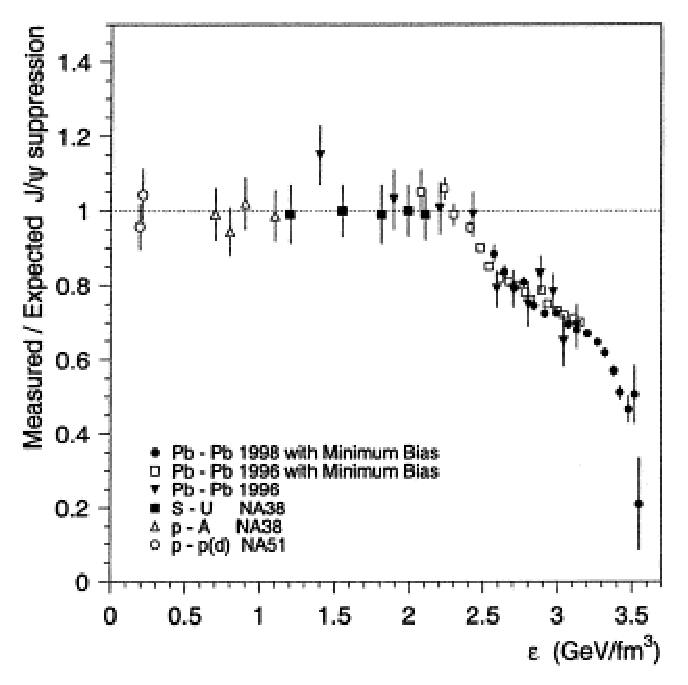
\includegraphics[width=6.6cm]{FigCap1/JPsiSuppressionNA50.eps}
  \includegraphics[width=7.2cm]{FigCap1/rhoMelting.png}
  \caption{Ratio between measured J/$\psi$ production and expected one in pp, p-A and A-A collisions as function of the energy density of the medium ~\cite{Abreu:2000ni}.}
  \label{fig:JPsiSuppressionNA50}
\end{figure}

\subsection{Chiral symmetry restoration}
\label{sec:ChiralSymm}
If, on one side, chiral symmetry restoration should play a role in the observed strangeness enhancement (see Sec.~\ref{subsec:StrangEnhancSPS}),
on the other hand, signatures of this effect could also be found in the mean and width values of mesons.
The $\rho$ meson was used from the very beginning as the test particle for in-medium modifications, due to the abundant production
of $\pi^+ \pi^- \rightarrow \rho$ and subsequent decay $\rho \rightarrow \mu^+ \mu^- $ with a short lifetime of 1.3 fm/c, then 
before thermal freeze-out. Fig.~\ref{fig:JPsiSuppressionNA50} (right) shows NA60 measurement of the 
low-mass di-muon pair invariant mass distribution for the
$\rho$ meson production, measured in In-In collisions at top SPS energy~\cite{Damjanovic:2005ni}. The rho is
clearly broadened in the fireball medium, while no sign of mass shift is observed, and the measurement
was found to be in good agreement with models describing an in-medium broadening scenario (Rapp/Wambach~\cite{Rapp:2012zq}).\\





Signals of a new state of matter had hence been found.
Moreover, the NA49 experiment gave the first indications that the fireball medium could be described by QCD hydrodynamics, with the measurement
of the so-called elliptic flow of pion and proton in semi-peripheral Pb-Pb collisions at top SPS energy~\cite{Alt:2003ab}. This observable, described in more detail in Sec.~\ref{sec:AnisotropicFlow}, is related with the
initial spatial anisotropy of the overlapping area of the two colliding nuclei, that is then converted into a final momenta anisotropy. Such a process is only possible if the fireball is guided by collective motion effects in a liquid-like medium with  small viscosity.
This effect and the experimental observations mentioned before will be deeper explored during the LHC phase. 
\begin{figure}[!b]
  \centering
  \includegraphics[width=12cm]{FigCap1/glauber.png}
  \caption{Schematic view of a nucleus-nucleus collision described in terms of the impact parameter b in the longitudinal (left) and transverse (right) plane.}
  \label{fig:image10}
\end{figure}

\section{Heavy-ion physics at the LHC}
We will go now through a revision of some of the most important results and open points regarding heavy-ion physics at the higher LHC energies. We will start with the characterization of the centrality of the collision, necessary to correctly interpret the properties of the so formed medium, to go then deeper inside the properties of the QGP.

\subsection{Collision Geometry and the Glauber Model}
In a collision of two nuclei, the impact parameter \textit{b}, i.e. the distance between the centers of the nuclei in the transverse plane of the collision, can span values from 0 to $R_1+R_2$, where  $R_1$ and  $R_2$ are the radii of the two nuclei. Small values of $b$ ($\lesssim$ 3.5 fm) imply large centrality in the collision. The impact parameter can not be measured directly, still it is possible to relate it to observables as the particle multiplicity, the transverse energy or the number of spectator nucleons. 
The Glauber model is used to calculate such geometric quantities that characterize the collision, and that can be correlated with centrality~\cite{Miller:2007ri}.
The model provides a phenomenological description assuming the nucleus-nucleus collision a superposition of indipendent nucleon-nucleon collisions.
Under the assumptions that, (i) at sufficiently high energies, the nucleons inside the nuclei are essentially undeflected after the collision, (ii) the nucleons move independently in the nucleus, (iii) protons and neutrons are indistinguishable and (iv) the radius of the nucleus is large compared to the extent of the nucleon-nucleon force, we can define the thickness functions of nuclei A, B for a certain value of impact parameter $b$ (see Fig.~\ref{fig:image10}):
\begin{equation}
T_i(\vec s) = \int\,dz \rho_i(\vec s,z).
\end{equation}
The thickness function is related to the nuclear density function $\rho$. The nuclear density is usually parameterized by a Woods-Saxon or 2-parameter Fermi distribution:
\begin{equation}
\rho (r) = \rho_0 \frac{1+w(r/R)^2}{1+{\rm exp}(\frac{r-R}{a})},
\end{equation}
where $\rho_0$ is the nuclear density in the center of the nucleus, $R = (6.62 \pm 0.06)$ fm is the radius parameter of the ${}^{208}$Pb, $a = (0.546 \pm 0.010)$ is the skin thickness of the Pb nucleus and $w$ characterizes deviations from a spherical shape ($w=0$ for Pb). The nuclear overlap function is then defined as:
\begin{equation}
T_{AB} = \int \,d^2s T_A(\vec s)T_B(\vec s - \vec b)
\end{equation}
and it gives the probability for two incoming nucleons inside two nuclei with impact parameter \textit{b} to be in the same area unity $d^2s$ on the transverse plane.
By considering the mean of a binomial distribution, the average number of binary nucleon-nucleon collisions $\langle N_{coll}\rangle$ as a function of the impact parameter \textit{b} can then be written as:
\begin{equation}
\langle N_{coll}\rangle = AB \times T_{AB}(b)\; \sigma^{inel}_{NN}.
\end{equation}
The number of participant nucleons in the collisions (nucleons of target and projectile that interact) can be obtained as:
\begin{equation}
\begin{aligned}
N_{part} (b) &= \int A \; T_A(\vec{s}) [1- (1- \sigma_{inel} T_B(\vec{b}-\vec{s}))^B]d^2s \\
& + \int B \; T_B(\vec{b}-\vec{s}) [1- (1- \sigma_{inel} T_A(\vec{s}))^A]d^2s.
\end{aligned}
\end{equation}
It is possible to demonstrate that the inelastic cross-section for a collision between two nuclei (A and B), depending on the impact parameter in a certain centrality range ($0 < b < b_c$) and using the Glauber model geometry, is:
\begin{equation}
\label{eq:sigmaABGlauber}
\sigma_{AB}(b_c) = \int_0^{b_c} 2\pi b\,db [1 - (1 - \sigma^{inel}_{NN}T_{AB}(b))^{AB}]. %\simeq \int_0^{b_c} 2\pi b\,db \cdot AB\cdot T_{AB}(b)  \sigma^{inel}_{NN}.
\end{equation}
\begin{figure}[!t]
\centering
\includegraphics[width=7cm]{FigCap1/Glauberimpactpar.pdf}
\includegraphics[width=7cm]{FigCap1/GlauberNpart.pdf}
\caption{Left: impact parameter distribution obtained from Glauber MC simulations for Pb-Pb collisions at $\sNN = 2.76$ TeV. Right: the corresponding $N_{\rm part}$ distributions for different intervals of impact parameter values.}
\label{fig:glaubMC}
\end{figure}
Finally the centrality can be defined as the percentile $c$ of the collisions in a given range of the impact parameter $b_{min}<$ b $<b_{max}$ (see Fig.~\ref{fig:glaubMC}), that is obtained as a fraction of the total nuclear interaction cross section $\sigma_{AB}$ by integrating on the impact parameter distribution $d\sigma_{AB}/db'$ as follows:
\begin{equation}
c=\frac{1}{\sigma_{AB}}\int_{b_{min}}^{b_{max}} \frac{d\sigma_{AB}}{db'}db'.
\end{equation}
In Chapter 3, more details will be given about the calculation of N\textsubscript{part} and  N\textsubscript{coll} for centrality determination in the ALICE experiment.
\iffalse
Two experimental observables related to the collision geometry are the average charged-particle multiplicity N\textsubscript{ch} and the energy carried by particles and deposited in the Zero-Degree Calorimeters (ZDC), called the zero-degree energy E\textsubscript{ZDC}. The average charged-particle multiplicity is assumed to decrease monotonically with increasing impact parameter. 
Therefore, the centrality of a collision could be defined as the percentile of the hadronic cross section corresponding to a particle multiplicity above a given threshold N$^{THR}_{ch}$ as follows:
\begin{equation}
c\sim \frac{1}{\sigma_{AA}}\int_{ N^{THR}_{ch}}^{\infty} \frac{d\sigma}{dN'_{ch}}dN'_{ch}
\end{equation}
The second experimental observable, the energy deposited in the zero-degree calorimeters, E\textsubscript{ZDC}, is directly related to the number of spectator nucleons N\textsubscript{spec}, which constitute the part of the nuclear volume not involved in the interaction. Hovewer, centrality ranges can not be simply obtained via a slicing of the multiplicity distribution mainly because of the presence of a significant contamination of electromagnetic processes at low multiplicity and of inefficiencies of the minimum-bias trigger. To avoid this bias, a Glauber Monte Carlo, combined with a simple model for particle production, is used to simulate a multiplicity distribution (e.g. the amplitudes of the VZERO scintillators in fig. \ref{fig:glaubVZERO}) which is then compared to the experimental one. So, it is possible to associate a value of N\textsubscript{part}, N\textsubscript{coll} and $\langle T_{AA}\rangle$ for each centrality class \cite{centrality}.
\fi
\begin{figure}[!t]
  \centering
  \includegraphics[width=7cm]{FigCap1/dNchdEtaVsEnergy.pdf}
  \includegraphics[width=7cm]{FigCap1/dNchdEtaVsNpart.pdf}
  \caption{(Left) Charged particle pseudo-rapidity density per participant pair for pp and central AA collisions as function of center-of-mass energy, measured in different colliding systems~\cite{Adam:2015ptt}. The fit to the power law is shown as solid (A-A) and dashed (pp) lines, together with the uncertainties on the dependence (shaded bands). (Right) Centrality dependence of (d$\Nch$/d$\eta$)/($\langle N_{\rm part} \rangle/2$) for p-Pb and Pb-Pb collisions at $\sNN=5.02$ TeV~\cite{ALICE:2012xs,Adam:2015gka}, Pb-Pb collisions at $\sNN=2.76$ TeV~\cite{Aamodt:2010cz} and pp collisions at $\sqrt{s}=7$ TeV measured with ALICE.}
  \label{fig:dNchdEta}
\end{figure}

\subsection{Particle multiplicity and energy density}
The number of produced particles (multiplicity) is related to the density of the created medium. Particle multiplicity depends in fact both on the centrality and energy of the collision. This observable is usually presented as a pseudo-rapidity ($\eta = - ln(\tan(\theta/2))$ density of charged particles at mid-rapidity (d$\Nch$/d$\eta |_{\eta=0}$). This is useful to compare experimental results with different acceptances. Furthermore, particle density is usually divided by the average number of participating nucleon pairs to the collision ($\langle N_{\rm part}\rangle$/2), to be comparable with results at different energies and colliding systems. Latest measurements from ALICE in the 5\% most central Pb-Pb collisions at $\sNN = 5.02$ TeV found a density of charged particles at mid-rapidity $\langle $d$\Nch$/d$\eta \rangle = 1943 \pm 54$ and, normalised per participant pair, (d$\Nch$/d$\eta$)/($\langle N_{\rm part} \rangle/2$) $ = 10.1 \pm 0.3$~\cite{Adam:2015ptt}.  
The left panel of Fig.~\ref{fig:dNchdEta} presents (d$\Nch$/d$\eta$)/($\langle N_{\rm part} \rangle/2$) as a function of the center-of-mass energy of the collision. The energy dependence of the charged multiplicity for central heavy-ion collisions can be fitted with a power law of the form $as^b$, where $b = 0.155 \pm$ 0.004~\cite{Adam:2015ptt}. The rise is much stronger than for pp collisions where $b = 0.103 \pm 0.002$, obtained from a fit to the same function. It can also be noticed that p-Pb values of (d$\Nch$/d$\eta$)/($\langle N_{\rm part} \rangle/2$) are included in the figure and lays on the pp curve, indicating that the strong rise in A-A collisions is not only related to the multiple interactions undergone by the participating nucleons, present in a p-A collision as well. The right panel of Fig.~\ref{fig:dNchdEta} shows instead the values of (d$\Nch$/d$\eta$)/($\langle N_{\rm part} \rangle/2$) as a function of the average number of participant nucleons in the collisions measured by ALICE in p-Pb~\cite{ALICE:2012xs} and Pb-Pb~\cite{Adam:2015ptt} collisions at $\sNN = 5.02$ TeV. The Pb-Pb measurements at $\sNN = 2.76 $ TeV~\cite{Aamodt:2010cz} are also shown, scaled by a factor of 1.2 (calculated from the observed $s^{0.155}$ dependence), as well as the pp measurements at $\sqrt{s}= 7$ TeV~\cite{Adam:2015gka} scaled by a factor of 1.13. The charged particle density per participant pair shows a strong dependence on $\langle N_{\rm part}\rangle$, decreasing of a factor 1.8 from most central collisions to peripheral ones. The measurement of particle production per participant pair can be used to constraint models describing particle production in heavy-ion collisions with different mechanisms. Among the others, theoretical calculations that are based on gluon saturation (rcBK-MC~\cite{Albacete:2011fw}, Kharzeev, Levin and Nardi~\cite{Kharzeev:2004if} and Armesto, Salgado and Wiedemann~\cite{Armesto:2004ud}) can give a good description of data. They are based on the idea of some transverse momentum scale at which the gluon and quark phase space density saturates, thus limiting the number of produced partons and, hence, of particles in ion collisions with respect to pp collisions.  \\
The simplified Bjorken model~\cite{Bjorken:1982qr} can be used to give an idea of which are initial spatial energy densities for the values of $\langle$$\Nch$/d$\eta$$\rangle$ at hand:
\begin{equation}
\label{Bjorken}
\epsilon_{Bj} = \frac{\langle m_T\rangle}{\tau_f A}\frac{dN_{\rm ch}}{dy}
\end{equation}
where $\tau_f$ is the formation time of the secondary particles, A is the overlap area of the two colliding nuclei, $\langle m_T \rangle$ is the average transverse mass of the created particles defined as $m_{T} = \sqrt{m^{2}+\pt^2}$ and $y$ is the rapidity. Starting from the measured values of d$\Nch$/d$\eta$, it is possible to estimate the energy density of the medium created in the collision.
At top RICH energy (200 GeV), for the most central collisions, one obtains $\sim 5$ GeV/fm$^3$ at the conservative estimate for the formation time $\tau_f$ = 1 fm/c~\cite{Bjorken:1982qr}, well above the critical value predicted by lattice QCD for phase transition. For central Pb-Pb collisions at the LHC at $\sNN$ = 2.76 TeV the value of $\epsilon_{Bj}$ is much higher and is around $\sim 14$ GeV/fm$^3$~\cite{Chatrchyan:2012mb}.

\subsection{Hadron multiplicities and chemical freeze-out}
If a chemical and thermal equilibrium governs the fireball when it undergoes chemical freeze-out, the thermal nature of the partonic state can be expected to be imprinted in the final hadron abundances. Since, if these conditions occur, the behavior of the system at the equilibrium can be described via a statistical approach, a description of the final particle yields in terms of thermodynamical observables becomes appealing. Following the approach described in~\cite{BraunMunzinger:2003zd}, we can introduce the partition function Z($T,V,\mu_{Q}$), a function that allows for a quantitative description of the statistical properties (temperature $T$, volume $V$ and chemical potentials $\mu_{Q}$) of the equilibrated system.
\begin{figure}[!ht]
  \centering
  \includegraphics[width=12cm]{FigCap1/GCThermalFit_PbPb010.pdf}
  \caption{Grand Canonical thermal fit to ALICE 0-10\% Pb-Pb data at $\sqrt{s_{\rm NN}} = 2.76$ TeV~\cite{Floris:2014pta}. Excluded volume correction implemented in THERMUS and GSI with r = 0.3 fm, $\mu_{B}$ fixed to 0, $\gamma_{s}$ fixed to 1, $\gamma_{c}$ fixed to 20. }
  \label{fig:GCThermalFit_PbPb010}
\end{figure}

In the Grand Canonical (GC) ensemble, adapt to describe a system in which energy and charges are on-average conserved within the full volume, the partition function is:
\begin{equation}
  \label{eq:PartitionFunction}
Z^{\rm GC} (T, V, \mu_{Q}) = {\rm Tr}[e^{-\beta(H - \sum_{i}{\mu_{Q_{i}}Q_{i}})}],
\end{equation}
where $H$ is the Hamiltonian of the system, $Q_{i}$ are the conserved charges, $\mu_{Q_{i}}$ are the chemical potentials needed to guarantee charges conservation on the average in the whole system and $\beta = 1/T$ is the inverse temperature. At the leading order, the Hamiltonian of a hadron resonance gas with no interaction contains all the degrees of freedom of a confined, strongly interacting medium. Further corrections can be added by introducing hadron repulsions, generally Van der Waals-like interactions. The Hamiltonian term can be used then to describe a gas with a hadron mass spectrum containing mesons with masses below $\sim 1.5 \; \Gevcc$ and baryons with masses below $\sim 2\; \Gevcc$. In this mass interval, the hadronic spectrum is well known as well as the decay channels of resonances and particles. With these assumptions, the maximum temperature for which the model can be considered trustable is $\sim 200$ MeV. The GC partition function of a non-interacting system, like that of our hypothesis, is given by the product of the independent partition functions of all the hadronic species. In the logarithmic form we write:
\begin{equation}
  \label{eq:LnPartFunction}
{\rm ln} Z(T, V \vec{\mu}) = \sum_{i} {\rm ln} Z_{i} (T, V, \vec{\mu}),
\end{equation}
where $\vec{\mu} = (\mu_B, \mu_S, \mu_Q)$, with the chemical potentials $\mu_i$ related to the baryon number, strangeness and electric charge, and the sum is over all species $i$.
The density of particle $i$ can be obtained from Eq.~\ref{eq:LnPartFunction} as:
\begin{equation}
\label{eq:ParticleDensity}
n_{i} (T, \vec{\mu}) = \frac{\langle N_{i} \rangle}{V} = \frac{1}{V}\frac{\partial (T {\rm ln}Z_i^{GC})}{\partial \mu_i} = \frac{T g_{i}}{2\pi^{2}} \sum_{k=1}^{\infty} \frac{(\pm 1)^{k+1}}{k} \lambda_{i}^{k} m_{i}^{2}K_{2}(\frac{km_{i}}{T}),
\end{equation}
where (+) is for fermions and (-) for bosons, $g_{i}$ is the spin-isospin degeneracy factor, $\lambda_{i} = e^{Q_{i}\mu_{i}}$ is the fugacity term and finally $K_{2}$ is the modified Bessel function.
Further corrections to the particle density are necessary at high temperature ($\gtrsim 100 $ MeV) or density, where the contribution to the particle yield $N_{i}$ from resonances decay becomes dominant with respect to the thermal production of the specie. Other deviations from the GC description can be taken into account by introducing parameters for strange, charm or light quarks ($\gamma_{S}, \gamma_{C}$ and $\gamma_{q}$) production. For example, in case there is no thermalisation for the strangeness component in the medium, the factor $\gamma_{s}<1$ is needed, usually whenever the size of system is small (i.e. pp collisions) or at low energy. 
Similar explanation applies to $\gamma_{C}$, introduced for the charm content.
The usage of $\gamma_{q}$ is only applied in the so called non-equilibrium model SHARE~\cite{Petran:2013lja}. This model describes an expanding, super-cooled quark-gluon plasma which undergoes a sudden hadronization without further re-interactions.
Among the five parameters of Eq.~\ref{eq:ParticleDensity} ($T, V, \mu_B, \mu_S, \mu_Q$), up to three can be fixed with the knowledge of the experimental conditions of the initial state. The other two parameters can be obtained by fitting the measured particle yields. In Fig.~\ref{fig:GCThermalFit_PbPb010}, a Grand-Canonical thermal fit with three different models using T and V as free parameters is performed on the $y$-differential identified particle yields measured by ALICE in the 10\% most central Pb-Pb collisions at $\sqrt{s_{\rm NN}} = 2.76$ TeV~\cite{Floris:2014pta}. The fit quality is not fully satisfactory ($\chi^{2}/ndf \sim 2$), while it used to be of order 1 for RHIC energies~\cite{Andronic:2008gu}. The temperature, as parameter of the fit, results to be of the order of 155 MeV. 
The measured p and $\Xi$ yields have a bad agreement with the fit (2.5 and 2 $\sigma$ respectively). The measurements of resonances in central Pb-Pb collisions suggest elastic re-scattering in the late hadronic phases, that becomes quite important for pion production. If protons are excluded from the fits, the fit quality improves and the temperature goes up to $\sim$160 MeV (closer to RHIC results). Non-equilibrium models like SHARE describe most hadrons very nicely but overestimate the nuclei by almost an order of magnitude, while the equilibrium model predicts them very nicely. Other models suggest that a single freeze-out temperature is not enough to describe the data~\cite{Bellwied:2013cta}, but temperature for lighter and heavier quarks could be different. So far, the production mechanism is not yet clearly understood as well as how the temperature from the thermal fit relates to the QCD phase transition temperature.

\subsection{Collective flow and kinetic freeze-out}
The Flow is a collective phenomenon, which is observed as a collective motion pattern superimposed to the chaotic thermal motion of the partons inside the fireball. Its origin is related to the large pressures generated when compressing and heating nuclear matter. It is possible to distinguish between different types of flow. Mainly, one is interested in the radial and the anisotropic flows. %The radial flow is present for every centrality, but it is stronger for central collisions. The anisotropic flow, instead, characterizes more peripheral collisions. \\
\subsubsection{Radial flow}
For what concerns the particle production in pp collisions, following the approach in~\cite{Schnedermann:1993ws} we can treat the momentum spectrum of particles as radiated by a thermal source with temperature $T$:
\begin{equation}
\label{eq:ThermalSource}
E\frac{d^{3}n}{d^3p} = \frac{dn}{dy \; m_{T} dm_T\;d\Phi} = \frac{gV}{(2\pi)^3}E\;e^{-(E-\mu)/T},
\end{equation}
  where $g$ is the spin-isospin-degeneracy factor for the particle species, $\mu$ is the grand canonical potential $\mu = n\mu_{B}+ s\mu_S$, originating from the quantum numbers $b$ and $s$ for baryon and strangeness content, $y$ is the rapidity, $m_{T}$ the transverse mass and $\hbar = c = k_B = 1$. By integrating Eq.~\ref{eq:ThermalSource} over rapidity using the modified Bessel function $K_1$, we obtain the transverse mass spectrum $dn/(m_Tdm_T)$, which behaves asymptotically like a decreasing exponential for transverse masses larger than the source temperature: 
\begin{equation}
\label{eq:SpectraBZ}
\frac{dN}{m_T dm_T} = \frac{V}{2\pi^2} m_T K_1 (\frac{m_T}{T}) \xrightarrow{m_T \gg T} V^\prime \sqrt{m_T} e^{-m_T/T}.
\end{equation}
It has been experimentally verified in pp collisions the universality of the temperature $T$ of the exponential slope of Eq.~\ref{eq:SpectraBZ}. The physical interpretation of $T_{slope}$ is the temperature of the system at the thermal freeze-out. The universality of $T_{slope}$ for different particle species is commonly referred to as $m_{T}$-scaling. When moving to nucleus-nucleus collisions, a breaking of the $m_T$-scaling occurs at low $\pt$ and the slopes of the spectra are observed to decrease with increasing mass~\cite{Appelshauser:1998yb,Arnaldi:2007ru}. The effect is present for every centrality, but it is stronger for central collisions. The slope of the exponential law thus needs a correction of the form:
\begin{equation}
\label{eq:Tslope}
T_{slope} = T_{fo} + \frac{1}{2}m \beta_{\perp}^{2},
\end{equation}
where the second term accounts for the dependence on the mass and the velocity is related to the radial flow, i.e. the collective velocity arising from the expansion of the fireball. The first term still accounts for the Brownian motion of the particles, present in Eq.~\ref{eq:SpectraBZ}. This is the idea developed within the Boltzmann-Gibbs blast-wave model~\cite{Schnedermann:1993ws}, where the radial expansion velocity distribution $\beta_r(r)$ in the region \mbox{$0 \leq r \leq R$} is parametrized by the surface velocity $\beta_s$:
\begin{equation}
\label{eq:Br}
\beta_r (r) = \beta_s \Big(\frac{r}{R}\Big )^n,
\end{equation}
and $n$ is used to tune the shape of the spectra profile.
\begin{figure}[!t]
  \centering
   \includegraphics[height=7cm]{FigCap1/PionsPbPb5TeV.png}
%   \includegraphics[height=8cm]{FigCap1/BWfit.pdf}
  \includegraphics[height=6cm]{FigCap1/BWfit_BetaTplot.pdf}
 \caption{Left: $\pi$ spectra in different centrality classes in Pb-Pb collisions at $\sNN = $ 5.02 TeV~\cite{Jacazio:2017dvy}. Right: $T_{kin}$ vs $\beta_T$ for different colliding systems and energies~\cite{Jacazio:2017dvy}.}
  \label{fig:BWfit_BetaTplot}
\end{figure}
The observed particle spectrum results then from the summation of the spectra of individual thermal sources each boosted with the boost angle $\rho = \tanh^{-1}(\beta_r)$.:
\begin{equation}
\label{eq:BlastWave}
\frac{dN}{\pt d\pt d\phi dy}\propto \int_{0}^{R} r dr\;  m_{T}\;  K_{1} \; (\frac{m_{T} \cosh(\rho(r))}{T_{fo}})\;  I_{0}\; (\frac{\pt \sinh(\rho(r))}{T_{fo}}).
\end{equation}
It is a three parameters ($T_{fo}, \beta_s, n$) simplified hydrodynamical model.
The blast-wave fit to the measured spectra (an example for pion production in Pb-Pb collisions at $\sNN = $ 5.02 TeV is shown in Fig.~\ref{fig:BWfit_BetaTplot} left~\cite{Jacazio:2017dvy}) allows an estimate of the kinetic freeze-out temperature $T_{fo}$ and transverse velocity $\beta_{\perp}$.
Fig.~\ref{fig:BWfit_BetaTplot} (right) shows the latest ALICE results for the blast-wave parameters ($T_{kin}$ and $\beta_{\perp}$ in the figure) for different colliding systems and energies. Blast-Wave parameters in Pb-Pb collisions at $\sNN = 5.02$ TeV follow trends obtained at lower energy ($\sNN = 2.76$ TeV). The largest expansion velocity is for central Pb-Pb collisions, as well as the lowest temperature for the kinetic freeze-out.\\

\subsubsection{Anisotropic flow}
\label{sec:AnisotropicFlow}
The anisotropic flow is characteristic of non-central collisions, where the finite impact parameter creates a fireball with a geometrical anisotropy. Due to particle rescatterings during the system evolution, the initial spatial anisotropy is transferred to a final momentum-space anisotropy. No rescatterings during the system evolution or any delays in time of such interactions would lead to no momentum anisotropy in the final state or to a decrease in the elliptic flow signal. Hence, the characterization of anisotropic flow is important as it is sensitive to particle interactions very early in the system evolution. Informations of the medium like Equation of State, sound velocity or shear viscosity can be exctracted by a comparison of the measured anisotropic flow and hydrodynamic model calculations.
\begin{figure}[!ht]
  \centering
  \includegraphics[width=8cm]{FigCap1/elliptic_flow_3D_medium.png}
  \caption{Picture of a semi-peripheral collisions and the pressure gradients arising from a geometrical anisotropy.}
  \label{fig:elliptic_flow_3D_medium}
\end{figure}

The reaction plane is defined by the impact parameter itself and the beam line (xz plane in Fig.~\ref{fig:elliptic_flow_3D_medium}). If enough particle rescattering occurs, a larger pressure gradient in the reaction plane than perpendicular to it is expected. This generates an anisotropy in azimuthal distributions of the particle momenta with respect to the reaction plane, which can be detected in the measured particle azimuthal distributions. This distribution can be parametrized through a Fourier series decomposition:
\begin{equation}
\label{eq:FourierAzimuthExpansion}
E \frac{d^3N}{d^3p} = \frac{1}{2\pi} \frac{d^2N}{p_t dp_t dy} (1 + \sum_{n=1}^\infty 2v_n {\rm cos} (n(\phi - \Psi_r))),
\end{equation}
where $\phi$ is the azimuthal direction of the emitted particle and $\Psi_r$ denotes the (true) reaction plane angle.
In the formula, {\it v$_n$} are the Fourier coefficients, and they can be evaluated as $v_n = \langle cos(n(\phi - \Psi_r)) \rangle$, where $\langle \rangle$ indicates an average over all particles in all events with their azimuthal angle $\phi$ in a given rapidity and $p_t$ momentum at a fixed centrality. The sine terms vanish due to the reflection simmetry with respect to the reaction plane. {\it Direct} and {\it elliptic flow} are common terms for the first and the
second order Fourier coefficients respectively in the particle azimuthal distribution in Eq.~\ref{eq:FourierAzimuthExpansion}, but coefficients up to at least 6th order were measured at the LHC~\cite{ATLAS:2012at}. With the large amount of data provided by the LHC, it became accessible to study not only the on-average anisotropies but the event-by-event flow fluctuations~\cite{Aad:2013xma,Schukraft:2012ah}, to which higher Fourier coefficients were indeed found to be sensitive. Fig.~\ref{fig:vnHydro} shows the fit with viscous hydrodynamics calculations~\cite{Gale:2012rq} to the Fourier coefficients $v_n$ up to 5th order measured by ATLAS~\cite{ATLAS:2012at} (left panel) in Pb-Pb collisions at $\sNN = 2.76$ TeV and PHENIX~\cite{Adare:2011tg} and STAR~\cite{Pandit:2012mq} (right panel) in Au-Au collisions at $\sNN = 200 $ GeV. The value of the shear viscosity $\eta/s$ of the medium from the hydro fits in Au-Au collisions at top of RICH energy is 0.12, while the value for Pb-Pb collisions at the LHC at $\sNN = 2.76$ TeV is 0.2. This reveals a dependence of the shear viscosity on the temperature of the system.
\begin{figure}[!ht]
  \centering
  \includegraphics[width=15cm]{FigCap1/RICH_ATLAS_vn.png}
  \caption{Fourier components of collective flow, $v_n(\pt)$, Pb-Pb collisions at the LHC (left panel) and for Au-Au collisions at RICH (right panel), in comparison with viscous hydrodynamics calculations~\cite{Gale:2012rq}.}
  \label{fig:vnHydro}
\end{figure}
\begin{figure}[!ht]
  \centering
  \includegraphics[width=15cm]{FigCap1/v2IdentifiedParticles.pdf}
  \caption{Flow coefficient $v_2$ of $\pi^{\pm}, K^{\pm}, p(\bar{p})$ and $\Phi$ meson for 10-20\% (left) and 40-50\% (right)
collision centrality as function of $\pt$~\cite{Bertens:2017krr}. Statistical uncertainties are shown as bars and systematic uncertainties as boxes.}
  \label{fig:v2IdentifiedParticles}
\end{figure}
Fig.~\ref{fig:v2IdentifiedParticles} shows the $\pt$-differential $v_2$ of $\pi^{\pm}, K^{\pm}, p(\bar{p})$ and $\Phi$ meson for 10-20\% (left)
and 40-50\% (right) collision centrality~\cite{Bertens:2017krr}, measured by ALICE~\cite{Bertens:2017krr} in Pb-Pb collisions at $\sNN = 5.02$ TeV.
For $\pt < 2$ $\Gevc$, one can notice that the $v_2$ of the different species follows a mass-ordering, which is indicative of strong radial flow.
For 3 $< \pt < 8$ $\Gevc$, particles are grouped according to their valence quark content, which supports the
hypothesis of particle production via quark coalescence~\cite{Molnar:2003ff}. The non-zero $v_2$ at high $\pt$ is attributed to path-length dependent in-medium energy loss effects~\cite{Gyulassy:2000gk}. The $\Phi$ meson, with its mass close to proton mass, is a very good probe of quark scaling and mass ordering. Indeed, the $\Phi$-meson $v_2$ follows proton $v_2$ at low $\pt$, but pion $v_2$ at intermediate $\pt$. \\

\subsection{Jet quenching}
High-$\pt$ partons formed in the early collisions of quarks and gluons from the two nuclei fragment into collimated cascades of hadrons, that are called jets. 
While partons and produced jets propagate inside the hot and dense QGP, they loose energy because of interactions with the colored medium (jet quenching), primarily via gluon radiation and, to smaller extent, elastic scattering~\cite{Qin:2015srf}. The quantitative observation of energy loss carries important information about transport coefficients of the QGP (different for radiative or collisional processes). Energy loss ($\Delta E$) is expected to be dependent on the opacity (associated to the medium density and the interaction strength) and on the path length $L$ traversed by the parton inside the medium. Different models predict linear and quadratic dependences on $L$ of the energy loss for elastic~\cite{Thoma:1990fm} and radiative~\cite{Baier:1996sk} collisions respectively (a cubic dependence is predicted within the AdS/CFT framework). Furthermore, $\Delta E$ also depends on the color charge (different for quarks and gluons) and on the quark mass, as it will be discussed in Sec.~\ref{} focusing in more detail on the heavy flavour quarks.

\begin{figure}[!ht]
  \centering
  \includegraphics[width=10cm]{FigCap1/Scattering.png}
  \caption{Schematic illustration of high $\pt$ hadron production in high-energy nuclear collisions. }
  \label{fig:Scattering}
\end{figure}

In perturbative QCD, the production cross-section for a hadron $h$ from processes involving high-momentum transfer can be described by the convolution of the incoming parton distribution functions (PDFs) inside the nucleons, the hard partonic scattering cross-section and the final state fragmentation function (FFs):
\begin{equation}
\label{eq:QCDhardProduction}
\begin{split}
d\sigma_{pp\rightarrow hX} \approx \sum_{abjd}\int dx_a \int dx_b \int dz_j f_{a/p} (x_a, \mu_f) \; \otimes \;f_{b/p} (x_b, \mu_f) \;\otimes \\
d\sigma_{ab \rightarrow jd} (\mu_f,\mu_F,\mu_R) \otimes D_{j\rightarrow h} (z_j,\mu_F), 
\end{split}
\end{equation}
where $x_a$, $x_b$ are the initial momentum fractions carried by the interacting partons in the nucleons, $z_j = p_h/p_j$ is the momentum fraction carried by the final observed hadron. Then, $f_{a/p} (x_a, \mu_f)$ and $f_{b/p} (x_b, \mu_f) $ are the two parton distribution functions, $d\sigma_{ab \rightarrow jd} (\mu_f,\mu_F,\mu_R) $ is the differential cross-section for parton scattering process and $D_{j\rightarrow h} (z_j,\mu_F)$ is the fragmentation function for parton $j$ to hadron $h$, which represents the probability for a quark to hadronize into a hadron carrying a fraction $z$ of the quark momentum. Finally, $\mu_f$ and $\mu_F$ are the factorization scales and $\mu_R$ is the renormalization scale. The PDFs are measured at a given $Q^2$ in experiments of deep inelastic scattering and evolved to different energy scales using DGLAP equations~\cite{Altarelli:1977zs}. Fragmentation functions cannot be calculated with pQCD and are usually measured in $e^+e^-$ collisions.\\



When studying energy loss of jets and partons inside the QGP, one has to disentangle two separate effects. The first is that the PDFs of bounded nucleons are different from those of the free nucleons. The so-called cold nuclear matter (CNM) effects are a consequence of this in bounded nucleons. The second is that the parton travelling across the QGP experiences energy loss (hot nuclear matter effects) before fragmenting in the final state.
Thus taking into account both cold and hot nuclear matter effects, Eq.~\ref{eq:QCDhardProduction} becomes:
\begin{equation}
\label{eq:QCDwNuclEffects}
d\sigma_{AB\rightarrow hX} \approx \sum_{abjj\prime d} f_{a/A} (x_a) \; \otimes \;f_{b/B} (x_b) \;\otimes d\sigma_{ab\rightarrow jd} \otimes P_{j\rightarrow j\prime} \otimes D_{h/j\prime}(z_{j\prime}), 
\end{equation}
where the additional piece $P_{j\rightarrow j\prime}$ describes the effects of the hard parton $j$ interacting with the colored medium before fragmenting into hadrons. \\

The experimental observable used for the study of energy loss inside the QGP is the nuclear modification factor, defined as the ratio between the production of particles in nucleus-nucleus collisions and the one expected according to the binary scaling in nucleon-nucleon collisions:
\begin{equation}
\label{eq:Raa}
\Raa (\pt, y) = \frac{1}{N_{\rm coll}}\frac{d^2N_{\rm AA}/\pt dy}{d^2N_{\rm pp}/\pt dy},
\end{equation}
where $N_{\rm coll}$ is the number of interacting nucleons in the colliding nuclei.
It is necessary to disentangle between cold and hot nuclear matter effects to have access to the medium transport properties via measurements of the $\Raa$. Some of the measurements of energy loss of high-$\pt$ particles and jets at the LHC are presented below.

\subsubsection{High-$\pt$ hadrons}
Measurements of the nuclear modification factors in central heavy-ion collisions at four different center-of-mass energies, for neutral pions ($\pi^0$) (SPS~\cite{Aggarwal:2001gn,dEnterria:2004cly,Alt:2007cd}, RHIC~\cite{Adare:2012wg}), charged hadrons ($h^{\pm}$) (RHIC\cite{Adams:2003kv}), and charged particles (LHC~\cite{Abelev:2012hxa,Aad:2015wga,CMS:2012aa}), compared to predictions of two models from~\cite{Chien:2015vja,Xu:2015bbz} are presented in Fig.~\ref{fig:CMSRaa}. The LHC measurements at $\sNN = 2.76$ and 5.02 TeV show stronger suppression than SPS and RHIC measurements. CMS extended the measurement of the $\Raa$ up to 300 $\Gevc$, and the suppression in the high-$\pt$ region is found to be smaller with increasing $\pt$, demonstrating that even very energetic partons suffer energy loss in the medium. ALICE complements the picture down to $\pt = 0 \; \Gevc$, showing a perfect agreement with CMS and ATLAS in the medium-$\pt$ region.
\begin{figure}[!ht]
  \centering
  \includegraphics[width=8cm]{FigCap1/CMSRaa.pdf}
  \caption{Measurements of the nuclear modification factors in central heavy-ion collisions at four different center-of-mass energies at SPS~\cite{Aggarwal:2001gn,dEnterria:2004cly,Alt:2007cd}, RHIC~\cite{Adare:2012wg,Adams:2003kv}, and LHC~\cite{Abelev:2012hxa,Aad:2015wga,CMS:2012aa}, compared to predictions of two models from~\cite{Chien:2015vja,Xu:2015bbz}}
  \label{fig:CMSRaa}
\end{figure}
ALICE also measured the nuclear modification factor of identified particle species, that can further constraint the models. In Fig.~\ref{fig:PiKPRaa5TeV} the $\Raa$ of pions, kaons and protons measured in Pb-Pb collisions at $\sNN = 5.02$ TeV is shown, for different centrality classes. First, it has to be noticed that the suppression has a clear dependence on the collision centrality, since it becomes stronger in more central events, where the medium is more spatially extended, in consistency with the path-length dependence above discussed. A second observation from results in Fig.~\ref{fig:PiKPRaa5TeV} is that there is a mass ordering at low $\pt$ that is a direct consequence of the radial flow. At high $\pt$ instead, the suppression is similar for the three species, indicating that the medium at high $\pt$ affects the different species in a similar way. Different model calculations were compared to the $\Raa$ measured in different centrality classes by CMS~\cite{CMS:2012aa} and ALICE~\cite{Abelev:2012hxa} and allowed for an extraction of the transport coefficient~\cite{Baier:1996sk} $\hat{q} \approx 1.7-1.9$ GeV$^2/c$ illustrated in~\cite{Burke:2013yra,Liu:2015vna}. 
\begin{figure}[!ht]
  \centering
  \includegraphics[width=15cm]{FigCap1/KPiPRAA5TeV.pdf}
  \caption{Nuclear modification factor of pions, kaons and protons measured by ALICE in Pb-Pb collisions at $\sNN = 5.02$ TeV in different centrality classes~\cite{Jacazio:2017dvy}.}
  \label{fig:PiKPRaa5TeV}
\end{figure}

\subsubsection{Jets}
The interest in jet measurement with respect to single hadrons is that they allow for more differential studies, therefore are expected to put more stringent constraints on assumptions in models for jet energy loss. Experimental techniques are now able enough to clearly identify jets even in the fluctuating background of high-energy heavy-ion collisions. The interaction of the high-$\pt$ partons with the color field of the medium induces the radiation of (mostly) soft ($\omega \ll E_{L}$, $E_L$ being the energy of leading parton) and collinear ($k_{\perp} \ll \omega$) gluons. The transport equation of a jet in the medium is then more complex than that of single hadron, since not only the energy loss of the leading parton has to be kept into account, but also the radiated gluons can further re-scatter in the medium inside the jet cone. Thus the total energy inside the jet cone of radius $R$ at the time $t_f$ is:
\begin{equation}
\label{eq:EnergyJet}
E_{jet}(t_f,R) = E_L(t_f) +E_g(t_f,R),
\end{equation}
where $E_g$ is the energy of the radiated gluons, that is defined as:
\begin{equation}
\label{eq:Eg}
E_g(t_f,R) = \int_R d\omega dk^2_\perp \omega f_g(\omega,k^2_\perp,t_f),
\end{equation}
where $f_g(\omega,k_{\perp},t)$ is the double differential distribution of the accompanying gluons of the full jet. It can be obtained after solving the following transport equation for the distribution of radiated gluons:
\begin{equation}
\label{eq:RadGluonTransport}
\frac{df_g(w,k_{\perp},t)}{dt} = -\hat{e}\frac{\partial f_g}{\partial \omega} + \frac{1}{4}\hat{q}\nabla^2_{k_{\perp}}f_g + \frac{dN^{rad}_g}{d\omega dk^2_{\perp} dt}.
\end{equation}
The first and the second term in Eq.~\ref{eq:RadGluonTransport} describe the evolution of radiated gluons which can transfer energy into the medium via collisional processes (controlled by coefficient $\hat{e}$) and accumulate transverse momentum $k_\perp$ (coefficient $\hat{q}$). The last term accounts for additional gluon radiation coming from emission of the leading parton.\\
\begin{figure}[!ht]
  \centering
  \includegraphics[width=9cm]{FigCap1/ATLASjetsRaa.png}
  \caption{Jet $\RAA$ as a function of $\pt$ in different centrality
intervals in Pb-Pb collisions at $\sNN = 2.76$ TeV~\cite{Aad:2014bxa}. Each panel shows a different range in $|y|$.}
  \label{fig:ATLASjetsRaa}
\end{figure}
\begin{figure}[!ht]
  \centering
  \includegraphics[width=15cm]{FigCap1/ATLASdiijetGammaZ.png}
  \caption{$\frac{1}{N}\frac{dN}{dx_J}$distribution for reconstructed photon-jet events in Pb-Pb collisions at $\sNN = 2.76$ TeV compared to PYTHIA calculations~\cite{ATLAS-CONF-2012-121}. Different centrality classes are shown in each column, while the rows show results for two jet radii, R $= 0.2$ and R $=0.3$.}
  \label{fig:ATLASdijetAsymm}
\end{figure} 
Fig.~\ref{fig:ATLASjetsRaa} shows jet $\Raa$ measured by ATLAS as a function of $\pt$ in different centrality classes and different rapidity selections for the three panels~\cite{Aad:2014bxa}. The suppression has a clear dependence on the event centrality, while is quite flat versus $\pt$ in the analysed range from 40 to 400 $\Gevc$. The result confirms the strong suppression of $\Raa$ observed for charged hadrons in Pb-Pb collisions at the LHC and reveals that the medium is so opaque to quench even the most energetic jets. The azimuthal correlations of transverse energy of back-to-back jets constitute an other interesting observable to characterize the effect of jet-medium interaction. At the LHC energies, a large number of dijet from back-to-bak partons is observed to have an asymmetry in the energy of the reconstructed jet pair. This is understood in terms of different path lengths that the two partons has to traverse in the medium. In general, measurements of inclusive jets and dijet suffers the fact that leading jets experience themselves some energy loss, thus the energy of the jet is not fully defined. Using weak bosons (Z or W) or photons, that do not interact with the medium, to replace one of the two jets allows to fully calibrate the initial energy of the jet, as explained in ~\cite{Wang:1996yh}. Fig.~\ref{fig:ATLASdijetAsymm} shows the $\frac{1}{N}\frac{dN}{dx_J}$ distribution for reconstructed photon-jet events in Pb-Pb collisions at $\sNN = 2.76$ TeV compared to PYTHIA calculations, where $x_J = \pt^{jet1}/\pt^{jet2}$~\cite{ATLAS-CONF-2012-121}. Each column corresponds to different centrality classes, while the rows show results for two jet radii, R $= 0.2$ and R $=0.3$. In more peripheral collisions the $x_J$ distribution is peaked towards 1, thus meaning that higher $\pt$ dijets tend to be balanced in momentum. Moving towards more central events, the $x_J$ distribution appears flatter around $0.5 < x_J<1$, to eventually become peaked around $x_J \sim 0.5$ in the 10\% more central events.

% \begin{figure}[!ht]
%   \centering
%   \includegraphics[width=10cm]{FigCap1/CentralPbPbRatiosThermalModels.pdf}
%   \caption{Mid-rapidity particle ratios, compared to RHIC results~\cite{Abelev:2008ab,Adler:2003cb,Arsene:2005mr} and predictions from thermal models~\cite{Andronic:2008gu,Cleymans:2006xj} for central Pb-Pb collisions at the LHC (combined statistical and systematic errors)~\cite{Abelev:2012wca}. }
%   \label{fig:CentralPbPbRatiosThermalModels}
% \end{figure}
\subsection{Quarkonium suppression}
Quarkonium, the bound state of a $c\bar{c}$ (charmonium) or $b\bar{b}$ (bottomonium) pair, was proposed from the very beginning as one of the most powerful signatures of the QGP formation (see Sec.~\ref{sec:JPsiSuppression}). Clear signs of J$/\psi$ suppression were indeed measured at the SPS, as a consequence of the strong color field of the plasma~\cite{Abreu:2000ni}. Charmonium states were also expected to melt at different temperatures of the plasma, accordingly to their bounding energy, and the sequential melting was experimentally verified~\cite{Du:2015wha,Digal:2001ue}. What turned out to be unexpected when data at the higher LHC energies became available was the observed enhancement of J$/\psi$ production at low $\pt$ with respect to the references at lower energy. In Fig.~\ref{fig:RaaJPsi} ALICE measurements of J$/\psi$ $\Raa$ at $\sNN = 2.76$ TeV~\cite{Abelev:2013ila} and at $\sNN = 5.02$ TeV~\cite{Adam:2016rdg} are compared to measurements at RHIC~\cite{Adare:2011yf} at $\sNN = 200$ GeV. In the left panel of Fig.~\ref{fig:RaaJPsi} the $\Raa$ is presented as a function of the centrality and shows smaller suppression at the higher energies, where the measurement is $\pt$ integrated in the interval $\pt < 8 \Gevc$. The centrality dependence is similar at the two LHC energies, with a systematic difference by about 15\%, even if the effect is within the total uncertainty of the measurements. In the right panel of the same figure, the dependence on $\pt$ reveals this unexpected effect to characterize the only low-$\pt$ region, becoming less dominant with increasing $\pt$, where the suppression mechanism should dominate. CMS measured the J$/\psi$ $\Raa$ in the high $\pt$ region, up to $\pt = $ 30 $\Gevc$, confirming a striking difference with respect to the low $\pt$ and reaching a suppression of $\sim 0.3$ for the most central events~\cite{Khachatryan:2016ypw}. All these observations may be explained by a (re)generation effect, feasible at the LHC energies with the abundant production of $c\bar{c}$ pairs, that eventually do recombine after in-medium dissociation. An other observable that is sensitive to the production mechanisms is the elliptic flow $v_2$. If the J$/\psi$ is produced by coalescence of charm quarks, and the charm do thermalise in the medium, the meson should acquire a non-zero flow itself. A non-zero $v_2$ could also be observed in case of significant in-medium energy loss, thus the final $v_2$ may be an interplay of multiple effects. Fig.~\ref{fig:JPsi} presents recent measurements by ALICE of J$/\psi$ $v_2$ at forward and mid-rapidity in Pb-Pb collisions at $\sNN = 5.02$ TeV for semi-central events (20-40\% centrality class)~\cite{Acharya:2017tgv}, compared with some of the available theoretical models. At forward rapidity, the maximum $v_2$ is reached between $4 < \pt < 6\; \Gevc$, with a significance for non-zero $v_2$ larger than $6.6\sigma$. Model calculations that include (re)combination of thermalised charm and beauty quarks as source of J$/\psi$ production, together with a path-length dependent in-medium energy loss can reproduce the magnitude of the measurement, but fail in reproducing the shape at higher $\pt$, suggesting a missing mechanism in the model ({\it Du et al.} in Fig.~\ref{fig:JPsi}~\cite{Du:2015wha}). The model by {\it Zhou et al.}~\cite{Zhou:2014kka} includes, in addition to the cited components, a component from the modification of the quarkonium production in the presence of a strong magnetic field in the early stage of the heavy-ion collision~\cite{Guo:2015nsa}. The $v_2$ resulting from the different in-plane than out-of-plane survival probability of primordial J$/\psi$ is shown as dashed red and dash-dotted orange lines. At the LHC energies also the bottomonia states have become accessible, opening the way to precision study for the $\Upsilon$({\it n}S) family. Due to the large masses of $b$ quarks, effects of coalescence are expected to be of smaller impact with respect to the charmonium~\cite{Andronic:2015wma}. A suppression pattern is expected also for $b\bar{b}$ states, due to different binding energies of the bottomonium states. CMS measured the $\Raa$ of $\Upsilon$(1S), $\Upsilon$(2S) and $\Upsilon$(3S) as a function of the centrality (Fig.~\ref{fig:JPsi}, right) in Pb-Pb collisions at $\sNN = 2.76$ TeV~\cite{Khachatryan:2016xxp}. The $\RAA$ shows a suppression for the $\Upsilon$(2S) state (factor of 8), that is larger with respect to the $\Upsilon$(1S) state (factor of $\sim$ 2), while the suppression of the $\Upsilon$(3S) state is obtained as an upper limit. The measured suppression of the three $\Upsilon$ states is compatible with theoretical models of a sequential melting of quarkonium states in a hot medium~\cite{Khachatryan:2016xxp}.
%~\cite{Sirunyan:2016znt}
\begin{figure}[!ht]
  \centering
  \includegraphics[width=7cm]{FigCap1/RaaJPsiAlicePhenix.pdf}
  \includegraphics[width=7cm]{FigCap1/RaaJPsiAlicePhenixVsPt.pdf}
  \caption{Centrality (left) and transverse momentum (right) dependence of the J$/\psi$ $\RAA$ measured by ALICE in the 0-20\% most central Pb-Pb collisions at $\sNN = 2.76$ TeV~\cite{Abelev:2013ila} (blue) and at $\sNN = 5.02$ TeV~\cite{Adam:2016rdg} (red) compared to PHENIX~\cite{Adare:2011yf} results in the 0-20\% most central Au-Au collisions at $\sNN = 200$ GeV.}
  \label{fig:RaaJPsi}
\end{figure}

\begin{figure}[!ht]
  \centering
  \includegraphics[width=7cm]{FigCap1/JPsiV2Models.pdf}
  \includegraphics[width=6cm]{FigCap1/RaaUpsilonCMS.png}
  \caption{Left: inclusive J$/\psi$ $v_2(\pt)$ at forward and mid-rapidity for semi-central (20-40\%) Pb-Pb collisions at $\sNN =$ 5.02 TeV~\cite{Acharya:2017tgv}. Calculations from transports model by~\cite{Du:2015wha} and~\cite{Zhou:2014kka} are also shown. Right: nuclear modification factors for $\Upsilon$(1S) and $\Upsilon$(2S) meson production in Pb-Pb collisions measured by CMS, as a function of centrality.
The upper limit derived on the nuclear modification factor for $\Upsilon$(3S) is represented with an arrow in the centrality integrated panel on the right~\cite{Khachatryan:2016xxp}. }
  \label{fig:JPsi}
\end{figure}

\subsection{Latest discoveries in small systems}
In 2010 CMS discovered first signals of long-range rapidity correlations in pp collisions at $\sqrt{s} = $ 7 TeV~\cite{Khachatryan:2010gv}, an effect that resulted quite unexpected to be found in small systems, being rather more naturally related with the hot and dense matter formed in heavy-ion collisions. This observation pawed the way to search further evidences of collective behaviors that could indicate signatures of QGP even in the small systems. The interest in the angular correlations among particles lays in the possibility to reveal the underlying mechanisms of particle production. In~\cite{Khachatryan:2010gv}, CMS studied the two-dimensional $\Delta \eta$-$\Delta \phi$ correlation function, where $\Delta \eta$ is the difference in pseudo-rapidity, with $\theta$ the polar angle relative to the beam axis) between two particles and $\Delta \phi$ is the difference in their azimuthal angle $\phi$. We can define now two correlation functions, the first one, $S_N(\Delta \eta,\Delta \phi)$ for the signal distribution:
\begin{equation}
\label{SignalDistribution}
S_N(\Delta \eta,\Delta \phi) = \frac{1}{N(N-1)}\frac{d^2N^{signal}}{d\Delta \eta d\Delta \phi}
\end{equation}
and the second, $B_N(\Delta \eta,\Delta \phi)$, for the background distribution:
\begin{equation}
\label{BkgDistribution}
B_N(\Delta \eta,\Delta \phi) = \frac{1}{N^2}\frac{d^2N^{mixed}}{d\Delta \eta d\Delta \phi}.
\end{equation}
$S_N(\Delta \eta,\Delta \phi)$ can be determined by counting all particle pairs in each event within a multiplicity bin, using the weighting factor $N(N-1)$. $B_N(\Delta \eta,\Delta \phi)$ is obtained instead by correlating each charged particle of one event with every particle from a different event within the same multiplicity bin. Finally, the $\pt$-inclusive two-particle correlation, as a function of $\Delta \eta$ and $\Delta \phi$ is obtained as:
\begin{equation}
\label{CorrelationFnc}
R(\Delta \eta,\Delta \phi) = \Big \langle (\langle N \rangle -1) \Big (\frac{S_N(\Delta \eta,\Delta \phi)}{B_N(\Delta \eta,\Delta \phi)} -1\Big )\Big \rangle,
\end{equation}
where the average is made over all the multiplicity bins of the analysis. By using the ratio of $S_N(\Delta \eta,\Delta \phi)$ and $B_N(\Delta \eta,\Delta \phi)$, detector effects such as tracking inefficiencies, non-uniform acceptances, etc, are automatically corrected. In Fig.~\ref{fig:CMSLongRangeRidge_pp7TeV}, $R(\Delta \eta,\Delta \phi)$ is plotted for high-multiplicity events ($N_{tracks} > 110$) in pp collisions at $\sqrt{s} = $ 7 TeV, with an applied selection on $1 <\pt < 3\; \Gevc$. Several correlation structures are present. The narrow peak at $(\Delta \eta, \Delta \phi) \approx (0,0)$ is the contribution from jet-like particle production (near-side peak). The broad ridge around $\Delta \phi \approx \pi$ is due to the fragmentation of back-to-back jets (away-side ridge). The ridge-like structure that appears around $\Delta \phi \approx 0$ was instead unexpected, indeed never observed in two-particle correlations in pp data, neither in minimum-bias events nor in high-multiplicity low $\pt$ events. Simulations do not reproduce the observed structure, that seems to resemble hydrodynamic behaviors of heavy-ion collisions~\cite{Alver:2008aa,Alver:2009id,Abelev:2009jv}, and the physical origin is still not clear.
\begin{figure}[!ht]
  \centering
  \includegraphics[width=7cm]{FigCap1/CMSLongRangeRidge_pp7TeV.png}
  \caption{Two-particle correlation functions in $\eta$-$\phi$ for 7 TeV pp collisions, in high multiplicity events ($N_{trk}>110$), with 1 $< \pt < 3 \Gevc$~\cite{Khachatryan:2010gv}.}
  \label{fig:CMSLongRangeRidge_pp7TeV}
\end{figure}
From this first observation, many studies have been done to unravel the nature of the long-range near side peak. Correlations among several produced particles have been explored, since this allows to further suppress short-range particle correlations, such as jets or resonance decays, as well as further investigating the collective nature of the observed azimuthal correlations. One of the most used methods is the Q-cumulants method. Following the approach in~\cite{Bilandzic:2010jr}, the correlations of two, four and six particles are evaluated as:
\begin{equation}
\label{correlations}
\begin{aligned}
\langle \langle 2 \rangle \rangle &= \langle \langle e^{in(\phi_1 -\phi_2)} \rangle \rangle &\\
\langle \langle 4 \rangle \rangle &= \langle \langle e^{in(\phi_1 + \phi_2 -\phi_3 - \phi_4)} \rangle \rangle &\\
\langle \langle 6 \rangle \rangle &= \langle \langle e^{in(\phi_1 + \phi_2 +\phi_3 - \phi_4- \phi_5- \phi_6))} \rangle \rangle,&
\end{aligned}
\end{equation}
where $\phi_i$ are the azimuthal angles of the correlated particles in an event, $n$ is the harmonic number and $\langle \langle ... \rangle \rangle$ indicates the average over all combinations from all events in a given multiplicity range. The cumulants are obtained as follows:
\begin{equation}
\label{eq:cumulants}
\begin{aligned}
\begin{split}
c_n\{4\} &= \langle \langle 4 \rangle \rangle - 2 \times  \langle \langle 2 \rangle \rangle^2 \\
c_n\{6\} &= \langle \langle 6 \rangle \rangle - 9 \times  \langle \langle 4 \rangle \rangle \langle \langle 2 \rangle \rangle + 12 \times \langle \langle 2 \rangle \rangle^3.
\end{split}
\end{aligned}
\end{equation}
Finally the Fourier harmonics $v_n$ coefficients are obtained from cumulants in Eq.~\ref{eq:cumulants} as:
\begin{equation}
\begin{aligned}
v_n \{4\} = \sqrt[4]{-c_n\{4\}} \\
v_n \{6\} = \sqrt[6]{\frac{1}{4}c_n\{6\}}.
\end{aligned}
\end{equation}
\begin{figure}[!ht]
  \centering
  \includegraphics[width=15cm]{FigCap1/v2CumulantsCMS.png}
  \caption{$v_2^{sub} \{2\, |\Delta \eta| > 2\}$, $v_2 \{4\}$ and $v_2 \{6\}$  as a function of the multiplicity, in the interval $0.3 < \pt < 3 \Gevc$ and $|\eta| < 2.4$~\cite{Khachatryan:2016txc} measured by CMS, in pp, p-Pb and Pb-Pb collisions.}
  \label{fig:CumulantsCMS}
\end{figure}
In the left panel of Fig.~\ref{fig:CumulantsCMS}, the $v_2 \{4\}$ and $v_2 \{6\}$ measured by CMS in pp collisions at $\sqrt{s} = 13$ TeV are shown as a function of the particle multiplicity, in the interval $0.3 < \pt < 3 \; \Gevc$ and $|\eta| < 2.4$. The values of $v_2 \{4\}$ and $v_2 \{6\}$ are compatible among them, as also observed in p-Pb and Pb-Pb collisions shown in middle and right panels of the same Fig.~\ref{fig:CumulantsCMS}. This supports the idea of a collective behavior behind the long-range correlations observed in pp collisions. Besides, in Fig.~\ref{fig:CumulantsCMS} the $v_2^{sub} \{2$, $|\Delta \eta| > 2\}$, defined as $v_2$ from two-particle correlation after subtraction of jet correlations from low multiplicity events, is also shown. Some hydrodynamical models interpret the similar magnitude of $v_2 \{4\}$ and $v_2^{sub} \{2$, $|\Delta \eta| > 2\}$ in pp collisions as the consequence of smaller number of initial fluctuating source than in p-Pb and Pb-Pb collisions.\\
Recently, ALICE reported about the first observation of strangeness production enhancement in high-multiplicity pp collisions~\cite{ALICE:2017jyt}. As anticipated in~\ref{subsec:StrangEnhancSPS}, strangeness enhancement was originally proposed as a signature of the Quark-Gluon Plasma and verified to be even more pronounced for multi-strange baryons. The production of strange hadrons in heavy-ion collisions can be described using a grand-canonical statistical model and do not show a significant dependence on the collision centrality, if one exclude the very peripheral events. For the latter, the relative yield of strange particles to pions becomes very similar to what observed in pp collisions. In~\cite{ALICE:2017jyt}, ALICE presented the measurement of the production of primary strange ($K^0_S,\; \Lambda,\; \bar{\Lambda}$) and multi-strange ($\Xi^-,\; \Xi^+,\; \Omega^-,\; \Omega^+$) hadrons in pp collisions at $\sqrt{s} = 7$ TeV. Fig.~\ref{fig:StrangenessALICEpp} (left panel) shows the $\pt$-differential yields of $K^0_S,\; \Lambda + \bar{\Lambda},\; \Xi^- + \Xi^+,\; \Omega^- + \Omega^+$ at mid-rapidity, for a selection of classes of events with progressively lower multiplicity, indicated by roman numbers in bracket in the figure. It can be noticed that the $\pt$ spectra become harder as the multiplicity increases, and the hardening becomes stronger with increasing particle mass. This is a feature already observed in p-Pb collisions~\cite{Abelev:2013haa} and typically characterizing Pb-Pb collisions, where they are described in terms of relativistic hydrodynamical expansion. A simultaneous fit with the blast-wave model to all $\pt$ spectra in defined $\pt$ ranges allowed the extraction of the chemical freeze-out temperature $T_{fo} = 163 \pm 10$ MeV and the transverse velocity of the bulk $\langle \beta_{\perp} \rangle = 0.49 \pm 0.02$. The $\pt$ distribution were then fitted in their full $\pt$ range using a Tsallis-Lèvy function to obtain the $\pt$-integrated yields. Finally, the right panel of Fig.~\ref{fig:StrangenessALICEpp} shows the ratio of $\pt$-integrated hadron yields to the pion yields, as a function of the charged-particle multiplicity, together with the measurements in p-Pb ($\sNN = 5.02$ TeV) and Pb-Pb ($\sNN = 2.76$ TeV) collisions. Despite the different energy of the collisions, the ratios show a smooth increase from pp to most central Pb-Pb collisions, with the highest multiplicity points in pp being fully compatible with the magnitude of the enhancement in p-Pb at same multiplicity values or in most peripheral Pb-Pb collisions. This suggests that the mechanism of strangeness enhancement is rather related with the characteristics of the final state produced in the collisions, than the characteristics of the collision itself. Still, the physical mechanism remains unclear, since the available models fail in reproducing at the same time both the ratios in Fig.~\ref{fig:StrangenessALICEpp} and the $\pt$-integrated proton to pion ratios at mid-rapidity~\cite{ALICE:2017jyt}.
\begin{figure}[!ht]
  \centering
  \includegraphics[width=14cm]{FigCap1/StrangenessALICEpp.png}
  \caption{Left: $\pt$-differential yields of $K^0_S,\; \Lambda + \bar{\Lambda}, \Xi^- + \Xi^+,\; \Omega^- + \Omega^+$ at mid-rapidity, for a selection of classes of events with progressively lower multiplicity. The Tsallis-Lèvy fit is shown as dashed line. Right: $\pt$-integrated ratios of $K^0_S,\; \Lambda + \bar{\Lambda},\; \Xi^- + \Xi^+,\; \Omega^- + \Omega^+$ to pion yield ($\pi^- + \pi^+$) as a function of $\langle dN_{ch}/d\eta \rangle$ at mid-rapidity~\cite{ALICE:2017jyt}.}
  \label{fig:StrangenessALICEpp}
\end{figure}













